\documentclass[oneside, a4paper, onecolumn, 11pt]{article}

% Change this: Customize the title, author, advisor, abstract
\newcommand{\thesistitle}[0]{Reparametrizing ODE models by scaling}
\newcommand{\authorname}[0]{Milos Oundjian}

\newcommand{\supervisor}[0]{Gleb Pogudin}
\newcommand{\supervisorinstitution}[0]{LIX}

\newcommand{\abstracttext}[0]{
    In this thesis, we present a novel implementation of the Hubert and Labahn algorithm for scaling invariants and symmetry reduction in dynamical systems, utilizing the Julia programming language. Our work extends the algorithm's application to non-identifiable models, offering a tool for the simplification and analysis of complex ordinary differential equation (ODE) models prevalent in the natural sciences. By integrating this implementation with the ``StructuralIdentifiability.jl'' package, we aim to make it easier for scientist to access this algorithm, enabling researchers without extensive computational backgrounds to leverage model simplification and reparameterization techniques. This approach not only facilitates the numerical solution of intricate models but also contributes to a deeper understanding of the underlying principles governing natural phenomena.
}

\usepackage[
    left=2cm,top=2.0cm,bottom=2.0cm,right=2cm,
    headheight=17pt, % as per the warning by fancyhdr
    includehead,includefoot,
    heightrounded, % to avoid spurious underfull messages
]{geometry}

% Added package
\usepackage[utf8]{inputenc}

% Template packages
\usepackage[T1]{fontenc}
\usepackage{amstext}
\usepackage{amsmath}
\usepackage{amssymb}
\usepackage{url}
\usepackage{graphicx}
\usepackage{wrapfig}
\usepackage{enumerate}
\usepackage{paralist}
\usepackage{xspace}
\usepackage{xcolor}
% Replace obsolete times package with mathptmx
% \usepackage{times}
\usepackage{mathptmx}
\usepackage[colorlinks, linkcolor=blue]{hyperref}
\setlength {\marginparwidth}{2.0cm}
\usepackage{pdfpages}
\usepackage{fancyhdr} %% For changing headers and footers
\usepackage{titling}
\usepackage[nottoc, numbib]{tocbibind}

% Added packages
\usepackage[framemethod=tikz]{mdframed} % For better box in abstract
\usepackage{esdiff} % For differentials
\usepackage{enumitem} % For step by step methodology
\usepackage{float} % For putting images properly

% Commands
\newcommand{\Z}[0]{\mathbb{Z}}
\newcommand{\Zn}[1]{\mathbb{Z}^{#1}}
\newcommand{\Zmn}[2]{\mathbb{Z}^{#1 \times #2}}

\newcommand{\todo}[1]{
    \begin{mdframed}
        \textcolor{orange}{
        TODO: #1
        }
    \end{mdframed}
}

\begin{document}

\hspace{0pt}
\vfill

\begin{center}
    
\includegraphics[width=0.3\textwidth]{logo-EP-vertical}
    \vspace*{2em}

    {\large
        \textbf{\'Ecole Polytechnique}
        \vspace*{1em}

        \textit{BACHELOR THESIS IN COMPUTER SCIENCE}
        \vspace*{3em}

        {\Huge \textbf{\thesistitle}}
        \vspace*{3em}

        \textit{Author:}
        \vspace*{1em}

        \authorname{}, \'Ecole Polytechnique
        \vspace*{2em}

        {\textit{Advisor:}}
        \vspace*{1em}

        \supervisor{}, \supervisorinstitution{}
    }
    \vspace*{2em}

    \textit{Academic year 2023/2024}
\end{center}

\vfill
\hspace{0pt}

\newpage

\noindent\textbf{Abstract}

\begin{mdframed}
    \abstracttext{}
\end{mdframed}

\newpage

% Setting up the header
\pagestyle{fancy}
%\renewcommand{\headrulewidth}{0pt} % Remove line at top
%\renewcommand{\headrulewidth}{0.4pt}% Default \headrulewidth is 0.4pt
\lhead{\authorname}
%\chead{\acronym}
\rhead{\thesistitle}

\newpage
\tableofcontents
\newpage

% \pagenumbering{arabic}

\section{Introduction}

Differential equations are a fundamental part of many natural sciences. The fields of Biology and Chemistry use differential models for many things. However, computationally, differential equations are not very easy to solve. In 2013, Evelyne Hubert and George Labahn hypothesized (and maybe implemented I'm not sure I couldn't find their code) an algorithm that would allow simplification of differential equations in order to make them easier to solve.

In their paper ``Scaling Invariants and Symmetry Reductions of Dynamical Systems'' \cite{Hubert2013}, they discuss the theory behind the algorithm and how it can be implemented.

The main overarching goal of this thesis is to implement an algorithm using scaling invariants and symmetry reduction of dynamical systems to improve the efficiency of solving ODEs computationally. What this means is that given an ODE, say for example the predator-prey model given by the following set of equations:
\begin{align*}
    \diff{n}{t}
     & = n (r (1 - \frac{n}{K} - k \frac{p}{n + d})), \\
    \diff{p}{t}
     & = sp (1 - h \frac{p}{n})
\end{align*}

In order to do this, I implemented in Julia, the necessary functions, such as getting the HNF multipliers in both row and column form. Most of the references for this. These include the functions \cite{Hubert2013}

Furthermore, I was (hopefully) able to integrate this algorithm that I had implemented into a more overarching Julia library ``StructuralIdentifiability.jl''

% \subsection*{Notes from Week 1}

% The goal of this week was to get familiar with the algorithm I will be working on. To do this I read through the main paper I will be working on (http://hal.inria.fr/hal-00668882). My first goal was to understand what Hermitian Normal Forms (HNFs) were. So I read up on them. HNFs fall into two categories, row and column, and this paper requires the use of both. The first issue I encountered was that the library I was using (specifically the Nemo Julia package) did not have an implementation for the column HNF. So I had to come up with my own implementation of it. While at first I looked at the algorithm (Cohen's algorithm from A Course in Computational Algebraic Number Theory), I realized that from the function could be implemented directly using the current `hnf` and `hnf\_with\_transform` function that already existed.

\section{Background}

\subsection{Hermite Normal Forms and Hermite Multipliers}

\subsubsection{Hermite Normal Forms (HNFs)}

While different sources may have varying definitions of Hermite Normal Forms, (explain the wikipedia def vs sisrds def here), the

According to \cite[SISRDS]{Hubert2013}, an \(m \times n\) integer matrix \(H = [h_{i, j}]\) is said to be in \textit{column} Hermite Normal Form if there exists an integer \(r\) and a strictly increasing sequence \(i_1, \dots, i_r\) of pivot rows such that:
\begin{enumerate}[label=(\roman*)]
    \item The first \(r\) columns are non-zero;
    \item \(h_{k, j} = 0\) for \(k > i_j\);
    \item \(0 \le h_{i_j, k} < h_{i,j j}\) when \(j < k\).
\end{enumerate}

The authors give a similar definition for the \textit{row} Hermite Normal Form being defined as there existing an integer \(r\) and a strictly increasing sequence \(j_1, \dots, j_r\) such that:
\begin{enumerate}[label=(\roman*)]
    \item The first \(r\) columns are non-zero;
    \item \(h_{i, k} = 0\) for \(k > j_i\);
    \item \(0 \le h_{k, j_i} < h_{i, j_i}\) when \(i < k\).
\end{enumerate}

Note that in this definition has index (i) unchanged for both row and column hermite normal form, and this definition does not seem standard across all sources came across (example here is wikipedia).

The reason that we care so much about the differences between is that our algorithm uses both forms in its different stages and we need to be very careful about which one we choose.

\subsubsection{Hermite Multipliers}

Any integer matrix \(A\) can be transformed via integer row operations (respectively column) to obtain a unique row (respectively column) Hermite Normal Form matrix H. We can encode these row operations (respectively column) into a unimodular integer matrix \(V\) such that we have \(V \cdot A = H\) (respectively \(A \cdot V = H\)). This matrix V is sometimes called the Hermite transform. In this paper we will be following \cite{Hubert2013} and calling in the \textit{Hermite Multiplier} of \(A\).

\todo{Maybe add an example here}

\subsubsection{Algorithmically determining HNF and Hermite Multipliers}

There exists algorithms that can computer Hermite Normal Forms which can be found for example in \cite{cohen2013course}. The steps and complexity of this algorithm is discussed there as well. However, for the scope of this paper we will not discuss these algorithms in detail.

Effectively, we will use these algorithms as a part of our algorithm. To do this we give this algorithm a specification. The function we care about is in the Julia library \texttt{Nemo.jl} and is called \texttt{hnf\_with\_transform}. The specification of this function is as follows:
\begin{figure}[H]
    \centering
    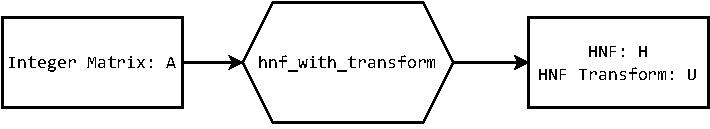
\includegraphics{images/diagram1.pdf}
    \caption{Existing Algorithm Specifications}
    \label{fig:existingalgo}
\end{figure}
\todo{Improve this figure to show that it is using row form}

This means that in our algorithm, we already have a tool that allows us to calculate row Hermite Normal Form. What we need to do is to find a way to use this tool, for example by doing matrix operations on the input matrix \(A\) and on the result from using the function \texttt{hnf\_with\_transform} to be able to create a new function that taking input matrix \(A\), returns the column hermite normal form of \(A\). In the next section we will show how we are able to do this and prove our new method.

The algorithm we implemented is as follows. It takes as input an \(m \times n\) integer matrix \(A\) and returns \(H, V\) where \(H\) is the Hermite Normal Form of \(A\) and \(V\) is the Hermite multiplier.
\begin{enumerate}
    \item Reverse the rows of \(A\).
    \item Transpose \(A\).
    \item Get the Hermite Normal Form of the new \(A\) and its transpose and its 
\end{enumerate}

\subsubsection{Practical Implementation}

There exists open source libraries that implement the algorithms to calculate the HNF form of a given matrix. For the purpose of this algorithm I have chosen to use the impl

\todo{Proof}


\subsection{Scalings}

A scaling is an operation on the differential equation that changes the

\section{Implementation}

% TODO: This is work in progress

In this section I will explain with an example the full methodology of the algorithm. The example I use is the the Schackenberg Model for a simple chemical reaction with limit cycle as shown in example 7.4 of \cite{Hubert2013}. The equation for this model is as follows.
\begin{align*}
    \diff{x}{t}
     & = a - kx + hx^2y \\
    \diff{y}{t}
     & = b - h x^2 y
\end{align*}

I explain the process to work on this from now on.

\begin{enumerate}[label=Step \arabic*:]
    \item Form the function \(F\) with the Laurent polynomials of the differential equations.
\end{enumerate}

\subsection{Example Implementation 1}

\subsection{Example Implementation 2}

\newpage
\bibliographystyle{plain}
\bibliography{main}

\newpage
\appendix

\section{Appendix}
\label{sec:appendix}

\end{document}
